%%%%%%%%%%%%%%%%%%%%%%%%%%%%%%%%%%%%%%%%%%%%%%%%%%%%
%%% Template criado por Jean Pimenta
%%%                v0.1
%%%      youtube.com/jeanpimenta
%%%     www.jeanpimenta.com/latex/
%%%     
%%%
%%% Todo o projeto foi compilado com XeLaTeX.
%%%
%%% Chamados de pacotes e definições se encontram
%%% na pasta preâmbulo dentro do projeto.
%%%
%%%%%%%%%%%%%%%%%%%%%%%%%%%%%%%%%%%%%%%%%%%%%%%%%%%%

\documentclass[12pt,a4paper,oneside]{article}

\usepackage{graphicx}
\usepackage{booktabs}
\usepackage{adjustbox}

\usepackage{caption}
% Documentação do pacote caption
% http://linorg.usp.br/CTAN/macros/latex/contrib/caption/caption-eng.pdf
%
% O uso de caption não deve ser feito com a classe memoir
\captionsetup{
	format=plain,
	font=small,
	labelfont=bf,
	figurewithin=section}
\captionsetup[figure]{name=Fig.}
\captionsetup[table]{name=Tab.}

%\makeatletter
%\counterwithout{figure}{chapter}
%\counterwithout{table}{chapter}
%\renewcommand{\figurename}{Figura}
%\renewcommand{\tablename}{Tabela}
%\makeatother


\begin{document}

\begin{minipage}{\textwidth}
\centering
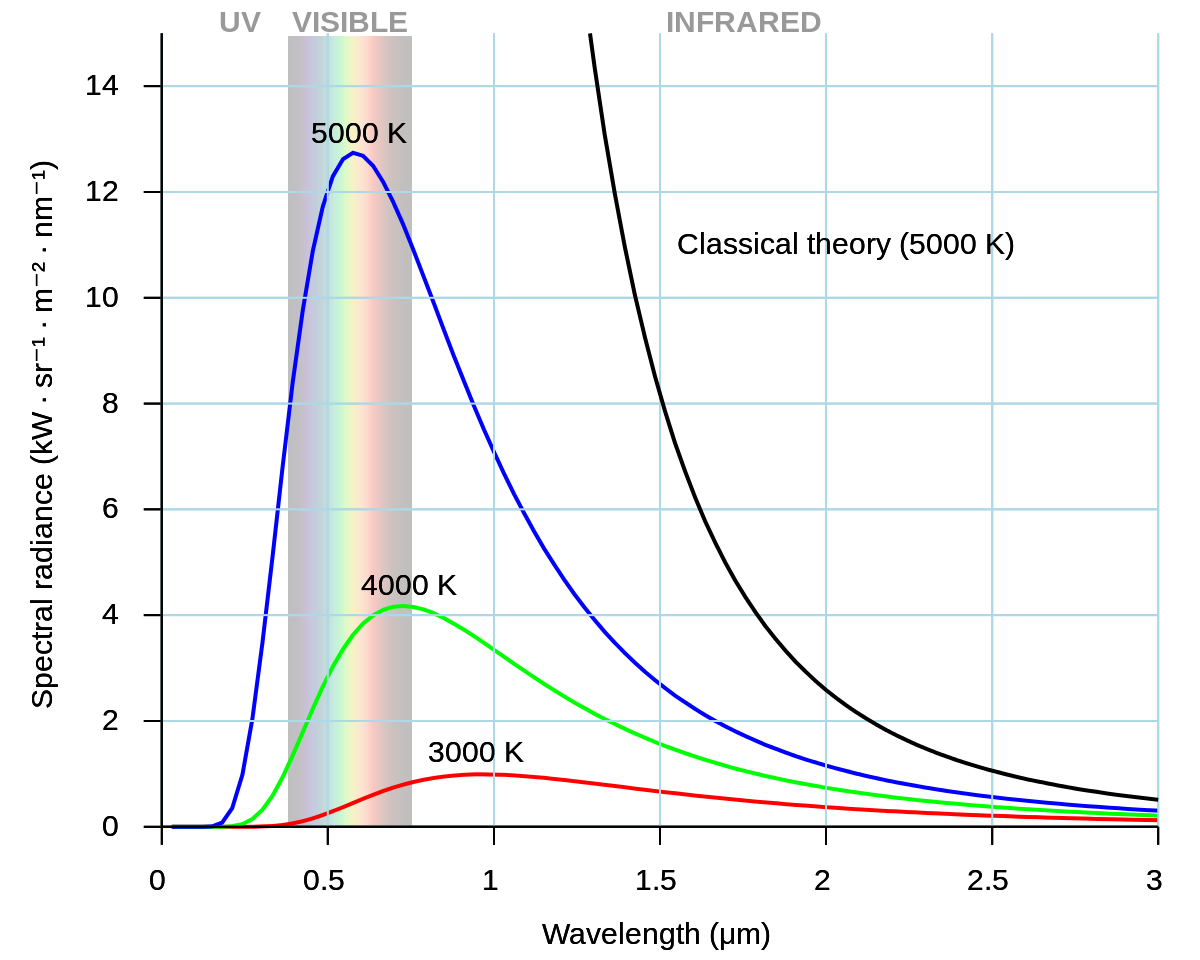
\includegraphics[scale=0.3]{figuras/Fig01}
\captionof{figure}{Título da Figura}
\end{minipage}

\vspace{30mm}

\begin{minipage}{\textwidth}
	\centering	
	\captionof{table}{Tabela 01}
	\small\setlength{\tabcolsep}{3pt}
	\begin{tabular}{l@{\hspace{6pt}} *{22}{c}}
	\toprule
	\bfseries Tipo & \multicolumn{22}{c}{\bfseries Medidas} \\
	\cmidrule(l){2-23}
	& 1 & 2 & 3 & 4 & 5 & 6 & 7 & 8 & 9 & 10 & 11 & 12 & 13 & 14 & 15 & 16 & 17 & 18 & 19 & 20 & 21 & 22 \\
	\midrule
	\bfseries A
	& 33 & 33 & 33 & 33 & 33 & 33 & 33 & 33 & 33 & 33 & 33
	& 33 & 33 & 33 & 33 & 33 & 33 & 33 & 33 & 33 & 33 & 33 \\
	\bfseries B
	& 33 & 33 & 33 & 33 & 33 & 33 & 33 & 33 & 33 & 33 & 33
	& 33 & 33 & 33 & 33 & 33 & 33 & 33 & 33 & 33 & 33 & 33 \\
\bottomrule
\addlinespace
\multicolumn{23}{l}{A: Número total de observações}\\
\multicolumn{23}{l}{B: Número de acontecimentos}
\end{tabular}
\end{minipage}

\end{document}